%%%%%%%%%%%%%%%%%%%%%%%%%%%
% Práctica 7:  Codelab Persistencia de datos
% @uthor: Ana del Carmen Santana Ojeda
% @date: 05/11/2023
%%%%%%%%%%%%%%%%%%%%%%%%%%%
% Estructura basica de la pagina
\documentclass[a4paper]{article}
\usepackage[utf8]{inputenc}
\usepackage[spanish]{babel}
\usepackage{fancyhdr} %Definimos el estilo de página

% Paquetes adicionales
\usepackage{graphicx,efbox}
\usepackage[headsep=0.2cm]{geometry}
\usepackage[most]{tcolorbox}
\newcommand{\MYhref}[3][black]{\href{#2}{\color{#1}{#3}}}
\usepackage[hyperindex=true, colorlinks=true, linkcolor=black, breaklinks=true, urlcolor=black, citecolor=black, anchorcolor= black]{hyperref}


% Agrega el paquete para personalizar el índice
\usepackage{tocloft}

% Personaliza la apariencia de la entrada "Bibliografía" en el índice
\renewcommand{\cftsecleader}{\cftdotfill{\cftdotsep}}
\renewcommand{\cftsecafterpnum}{\vspace{0.5\baselineskip}}

% Variable de entorno de fecha
\newcommand{\dateToday}{22 de octubre de 2023}

% Variable de imagenes
\newcommand{\logoULPGC}{imagenes/ulpgc.png}
\newcommand{\portada}{imagenes/portada.png}
\newcommand{\busSchedule}{imagenes/busSchedule.png}
\newcommand{\dessert}{imagenes/dessert.png}

%Cambio indice
\addto\captionsspanish{\renewcommand{\contentsname}{Índice}}

\setlength{\headheight}{ 40.2pt}
\pagestyle{fancy}
\lhead{\includegraphics[width=5cm]{\logoULPGC}}\rhead{
\includegraphics[height=1cm]{imagenes/portada.png}}

\geometry{a4paper, total={170mm,257mm}, left=35mm, top=20mm, right=35mm}

\begin{document}
    %%%%%%%%%%%%%%%%%%%%%%%%%%%%%%%%%
    %%   Portada del documento
    %%%%%%%%%%%%%%%%%%%%%%%%%%%%%%%%%
    \begin{titlepage}
        \centering
        \vspace*{2cm}
        \includegraphics[width=0.6\textwidth]{\logoULPGC}\par\vspace{1cm}
    
        {\scshape\textbf{\LARGE Práctica 7}}\par
        \vspace{0.6cm}
        {\bfseries}{\Huge Persistencia de datos}
        \vspace{2cm}
    
        \centering
        \fbox{
\includegraphics[width=\textwidth, height=8cm, keepaspectratio]{\portada}}
        \vspace{1cm} 
        
        \begin{tcolorbox}[colback=green!5!white,colframe=white!50!black]
            \centering \Large Programación de Aplicaciones Móviles Nativas \par
            \dateToday
        \end{tcolorbox}

        \vspace{1cm}        
        \begin{tcolorbox}[colback=green!5!white,colframe=white!75!black]
            Autora:
            \tcblower
            Ana del Carmen Santana Ojeda (ana.santana152@alu.ulpgc.es)
        \end{tcolorbox}
    \end{titlepage}
    
    \newpage
        
    %%%%%%%%%%%%%%%%%%%%%%%%%%%%%%%%%
    % Tabla de contenido de la pagina
    %%%%%%%%%%%%%%%%%%%%%%%%%%%%%%%%%
    \tableofcontents 
    
    \newpage

    %%%%%%%%%%%%%%%%%%%%%%%%%%%
    % Introduccion de la pagina
    %%%%%%%%%%%%%%%%%%%%%%%%%%%
    \section{Introducción}

    Esta actividad se centra en '\textbf{Persistencia de datos}' a través de tres cursos breves. El primer cursos, '\textbf{Introducción a SQL}', abarca los conceptos básicos de SQL, tal como sugiere su título. El segundo curso, '\textbf{Cómo usar Room para lograr la persistencia de datos}' explica el uso de la biblioteca \textbf{Room} para la creación y utilización de bases de datos, además realizaremos una app llamada '\textbf{Bus Schedule}'. El último minicurso se centra en la '\textbf{Cómo almacenar datos y acceder a ellos mediante claves con DataStore}', aprenderemos como \textbf{almacenar datos} y realizaremos una aplicación de '\textbf{Flight Search}'.
    
    \section{Enlace Github}
    %Enlace al repositorio de Git con el CodeLab
    \href{https://github.com/AnaSantana016/PAMN_G13/tree/Practica6}{Enlace del Github} 
    
    \section{Capturas del emulador}
    %Capturas de pantalla de la App en el emulador

    Como mencionamos en la introducción, de estos tres minicursos, dos de ellos incluyen dos proyectos cada uno. Uno de los proyectos se llama \textbf{'Bus Schedule'}.

    \begin{figure}[h]
        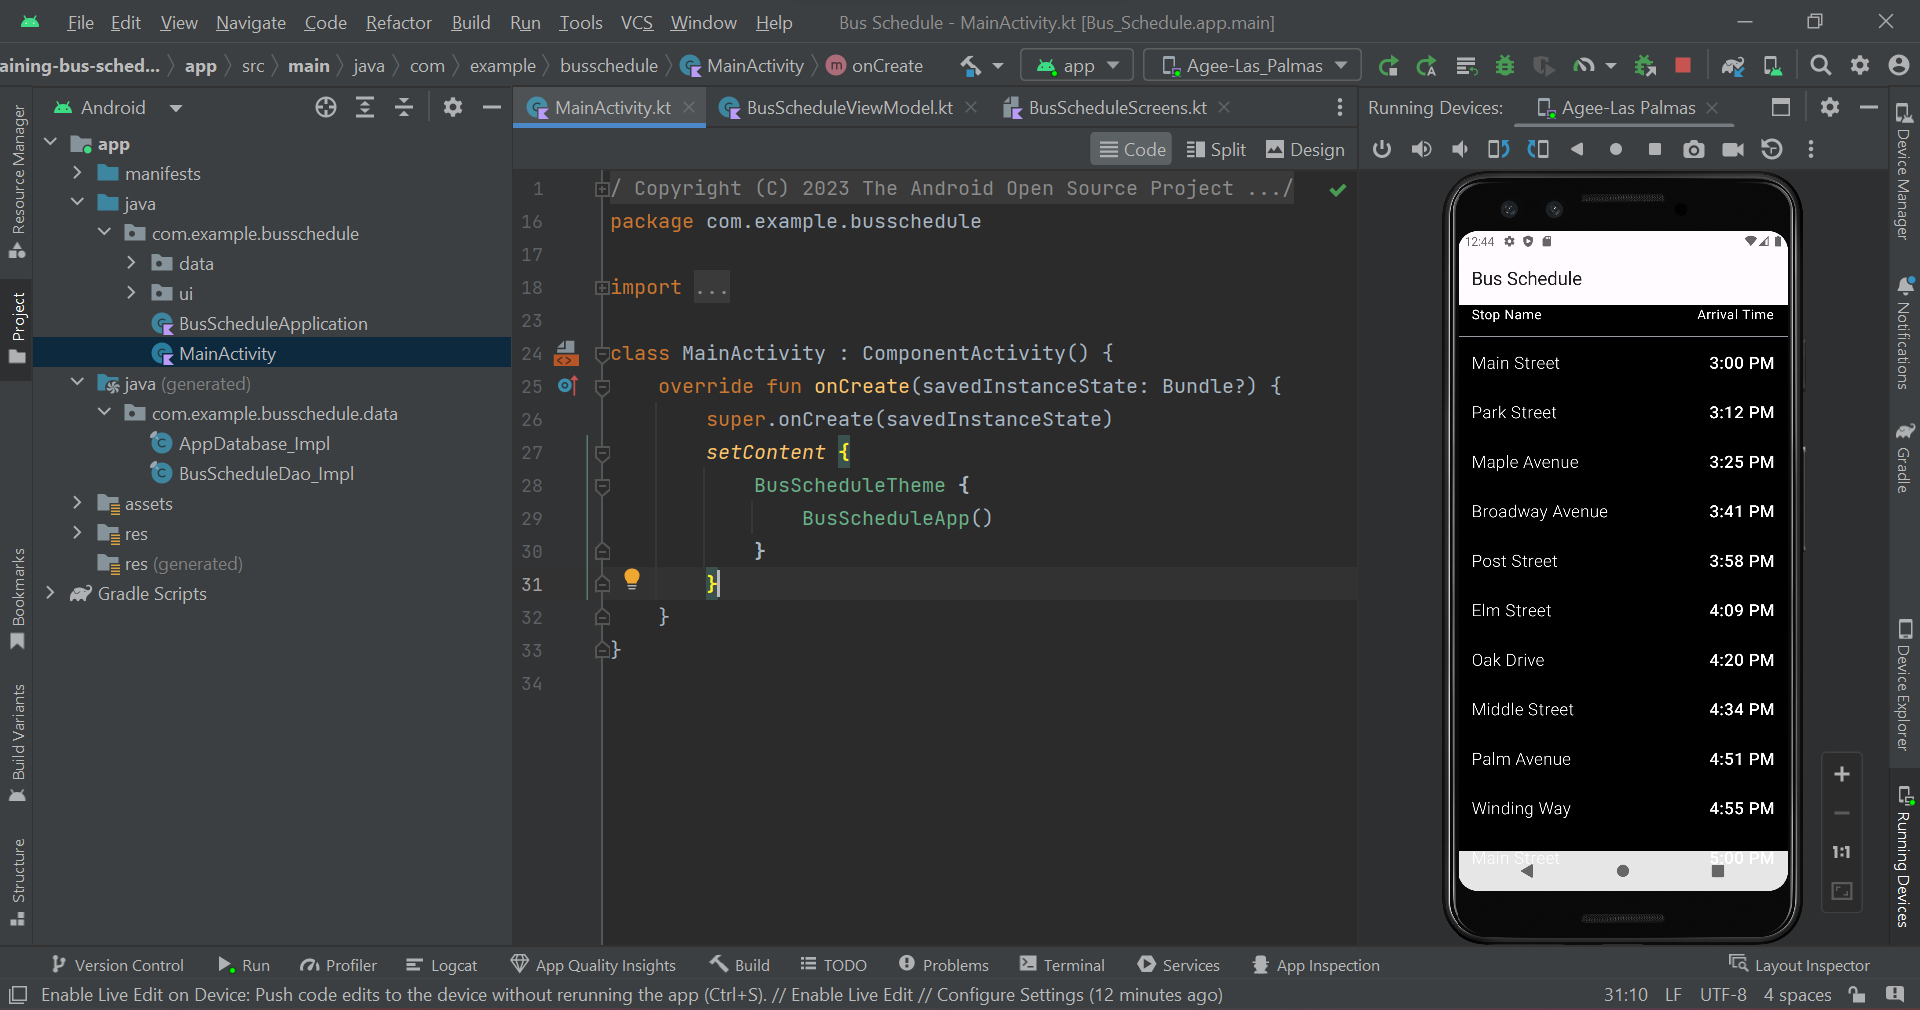
\includegraphics[width=\textwidth, height=8cm, keepaspectratio]{\busSchedule}
        \caption{Bus Schedule}
    \end{figure}

    Este proyecto consistía en aprender cómo \textbf{crear y utilizar base de datos con Room} en nuestro proyecto. Adicionalmente decidí cambiar el color de fondo a negro y la letras del contenido a blanco, como se puede apreciar en la Figura 1.

    \newpage
    
    El último proyecto que realizamos fue el de \textbf{'Flight Search'}, pero por falta de tiempo decidí modificar un proyecto que ya estaba hecho en el minicurso que se llama \textbf{'Dessert Release'}

    \begin{figure}[h]
        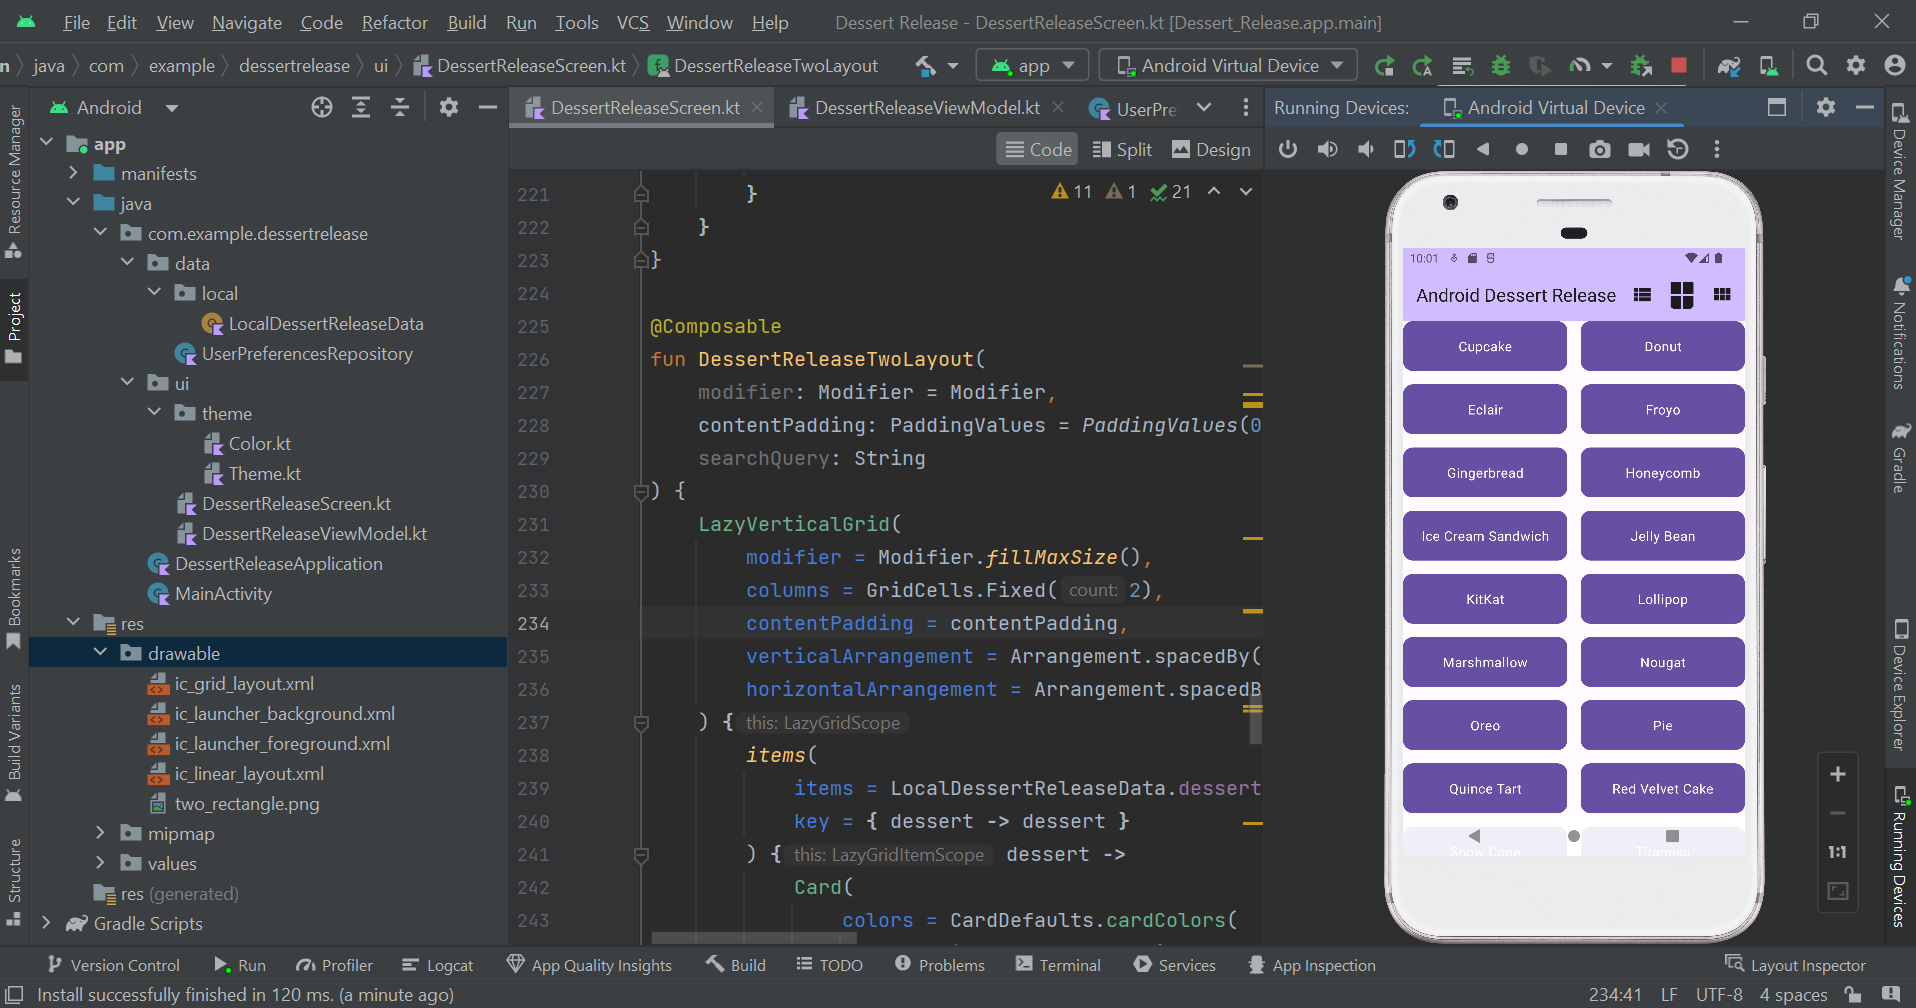
\includegraphics[width=\textwidth, height=8cm, keepaspectratio]{\dessert}
        \caption{Dessert}
    \end{figure}

    Como podemos observar en la Figura 2, consistía en \textbf{utilizar datastore} para que se te guarde el estado del icono que haya picado. El cambio que le hice fue añadir un icono más y cuando clicke en el te visualice dos columnas.
    
    \section{Opinion del codelab}

    En cuanto a los minicursos, lo vi \textbf{muchos más largos y a veces me perdía}.\vspace{0.3cm}
    
    El primer minicurso está muy bien explicado y ayuda a recordar conceptos que ya hemos tocado anteriormente en la universidad. El segundo minicurso también está bien explicado y es fácil de seguir, siento que he entendido bien cómo utilizar Room. En cuanto al último curso, es cierto que lo encontré más difícil y tengo la sensación de que no he aprendido mucho sobre DataStore.
    
\end{document}